{
\begin{figure}[ht!]
    \centering
    \begin{subfigure}[t]{0.3\textwidth}
        \centering
        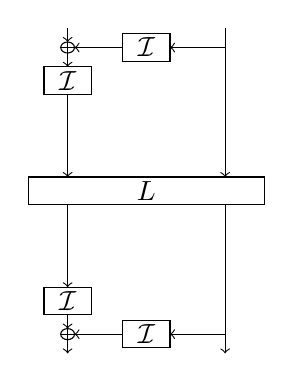
\begin{tikzpicture}[xscale=1.0, yscale=-0.35]
            \draw [->] (0,0) -- (0,0.5);
            \draw (0,0.7) ellipse (0.0875 and 0.2);
            \draw (0,0.5) -- (0,0.9);
            \draw (-0.0875,0.7) -- (0.0875,0.7);
            \draw (2,0) -- (2,0.7);
            \draw [->] (2,0.7) -- (1.3,0.7);
            \draw (0.7,0.2) rectangle (1.3,1.2) node[pos=0.5] {$\mathcal{I}$};
            \draw [->] (0.7,0.7) -- (0.0875,0.7);
            \draw [->] (0,0.9) -- (0,1.4);
            \draw (-0.3,1.4) rectangle (0.3,2.4) node[pos=0.5] {$\mathcal{I}$};
            \draw [->] (0,2.4) -- (0,5.4);
            \draw [->] (2,0.7) -- (2,5.4);
            \draw (-0.5,5.4) rectangle (2.5,6.4) node[pos=0.5] {$L$};
            \draw [->] (0,6.4) -- (0,9.4);
            \draw (-0.3,9.4) rectangle (0.3,10.4) node[pos=0.5] {$\mathcal{I}$};
            \draw [->] (0,10.4) -- (0,10.9);
            \draw (0,11.1) ellipse (0.0875 and 0.2);
            \draw (0,10.9) -- (0,11.3);
            \draw (-0.0875,11.1) -- (0.0875,11.1);
            \draw (2,6.4) -- (2,11.1);
            \draw [->] (2,11.1) -- (1.3,11.1);
            \draw (0.7,10.6) rectangle (1.3,11.6) node[pos=0.5] {$\mathcal{I}$};
            \draw [->] (0.7,11.1) -- (0.0875,11.1);
            \draw [->] (0,11.3) -- (0,11.8);
            \draw [->] (2,11.1) -- (2,11.8);
        \end{tikzpicture}
    \end{subfigure}
    \hspace{0.2cm}
    \begin{subfigure}[t]{0.3\textwidth}
        \centering
        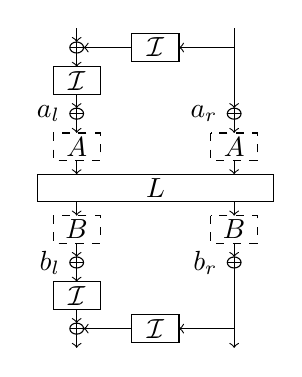
\begin{tikzpicture}[xscale=1.0, yscale=-0.35]
            \draw [->] (0,0) -- (0,0.5);
            \draw (0,0.7) ellipse (0.0875 and 0.2);
            \draw (0,0.5) -- (0,0.9);
            \draw (-0.0875,0.7) -- (0.0875,0.7);
            \draw (2,0) -- (2,0.7);
            \draw [->] (2,0.7) -- (1.3,0.7);
            \draw (0.7,0.2) rectangle (1.3,1.2) node[pos=0.5] {$\mathcal{I}$};
            \draw [->] (0.7,0.7) -- (0.0875,0.7);
            \draw [->] (0,0.9) -- (0,1.4);
            \draw (-0.3,1.4) rectangle (0.3,2.4) node[pos=0.5] {$\mathcal{I}$};
            \draw [->] (0,2.4) -- (0,2.9);
            \draw (0,3.1) ellipse (0.0875 and 0.2);
            \draw (0,2.9) -- (0,3.3);
            \draw (-0.0875,3.1) -- (0.0875,3.1);
            \draw (-0.0875,3.1) node[anchor=east] {$a_l$};
            \draw [->] (2,0.7) -- (2,2.9);
            \draw (2,3.1) ellipse (0.0875 and 0.2);
            \draw (2,2.9) -- (2,3.3);
            \draw (1.9125,3.1) -- (2.0875,3.1);
            \draw (1.9125,3.1) node[anchor=east] {$a_r$};
            \draw [->] (0,3.3) -- (0,3.8);
            \draw [dashed] (-0.3,3.8) rectangle (0.3,4.8) node[pos=0.5] {$A$};
            \draw [->] (2,3.3) -- (2,3.8);
            \draw [dashed] (1.7,3.8) rectangle (2.3,4.8) node[pos=0.5] {$A$};
            \draw [->] (0,4.8) -- (0,5.3);
            \draw [->] (2,4.8) -- (2,5.3);
            \draw (-0.5,5.3) rectangle (2.5,6.3) node[pos=0.5] {$L$};
            \draw [->] (0,6.3) -- (0,6.8);
            \draw [dashed] (-0.3,6.8) rectangle (0.3,7.8) node[pos=0.5] {$B$};
            \draw [->] (2,6.3) -- (2,6.8);
            \draw [dashed] (1.7,6.8) rectangle (2.3,7.8) node[pos=0.5] {$B$};
            \draw [->] (0,7.8) -- (0,8.3);
            \draw (0,8.5) ellipse (0.0875 and 0.2);
            \draw (0,8.3) -- (0,8.7);
            \draw (-0.0875,8.5) -- (0.0875,8.5);
            \draw (-0.0875,8.5) node[anchor=east] {$b_l$};
            \draw [->] (2,7.8) -- (2,8.3);
            \draw (2,8.5) ellipse (0.0875 and 0.2);
            \draw (2,8.3) -- (2,8.7);
            \draw (1.9125,8.5) -- (2.0875,8.5);
            \draw (1.9125,8.5) node[anchor=east] {$b_r$};
            \draw [->] (0,8.7) -- (0,9.2);
            \draw (-0.3,9.2) rectangle (0.3,10.2) node[pos=0.5] {$\mathcal{I}$};
            \draw [->] (0,10.2) -- (0,10.7);
            \draw (0,10.9) ellipse (0.0875 and 0.2);
            \draw (0,10.7) -- (0,11.1);
            \draw (-0.0875,10.9) -- (0.0875,10.9);
            \draw (2,8.7) -- (2,10.9);
            \draw [->] (2,10.9) -- (1.3,10.9);
            \draw (0.7,10.4) rectangle (1.3,11.4) node[pos=0.5] {$\mathcal{I}$};
            \draw [->] (0.7,10.9) -- (0.0875,10.9);
            \draw [->] (0,11.1) -- (0,11.6);
            \draw [->] (2,10.9) -- (2,11.6);
        \end{tikzpicture}
    \end{subfigure}
    \FigDef{propagation-affine}{Affine-equivalent structures.}
\end{figure}
}